\section[Fully-Implicit Model]{Solving a Problem Using a Fully-Coupled Model}\label{tutorial-coupled}

The process of setting up a problem using \Dumux can be roughly divided into four parts:
\begin{enumerate}
 \item A suitable model has to be chosen.
 \item The geometry of the problem and correspondingly a grid have to be defined.
 \item Material properties and constitutive relationships have to be selected.
 \item Boundary conditions and initial conditions have to be specified.
\end{enumerate}

The problem being solved in this tutorial is illustrated in Figure \ref{tutorial-coupled:problemfigure}. 
A rectangular domain with no flow boundaries on the top and on the bottom, which is initially saturated with oil, is considered. 
Water infiltrates from the left side into the domain and replaces the oil. Gravity effects are neglected here.

\begin{figure}[ht]
\psfrag{x}{x}
\psfrag{y}{y}
\psfrag{no flow}{no flow}
\psfrag{water}{\textbf{water}}
\psfrag{oil}{\textcolor{white}{\textbf{oil}}}
\psfrag{p_w = 2 x 10^5 [Pa]}{$p_w = 2 \times 10^5$ [Pa]}
\psfrag{p_w_initial = 2 x 10^5 [Pa]}{\textcolor{white}{\textbf{$\mathbf{p_{w_{initial}} = 2 \times 10^5}$ [Pa]}}}
\psfrag{S_n = 0}{$S_n = 0$}
\psfrag{S_n_initial = 0}{\textcolor{white}{$\mathbf{S_{n_{initial}} = 1}$}}
\psfrag{q_w = 0 [kg/m^2s]}{$q_w = 0$ $\left[\frac{\textnormal{kg}}{\textnormal{m}^2 \textnormal{s}}\right]$}
\psfrag{q_n = -3 x 10^-4 [kg/m^2s]}{$q_n = -3 \times 10^{-2}$ $\left[\frac{\textnormal{kg}}{\textnormal{m}^2 \textnormal{s}}\right]$}
\centering
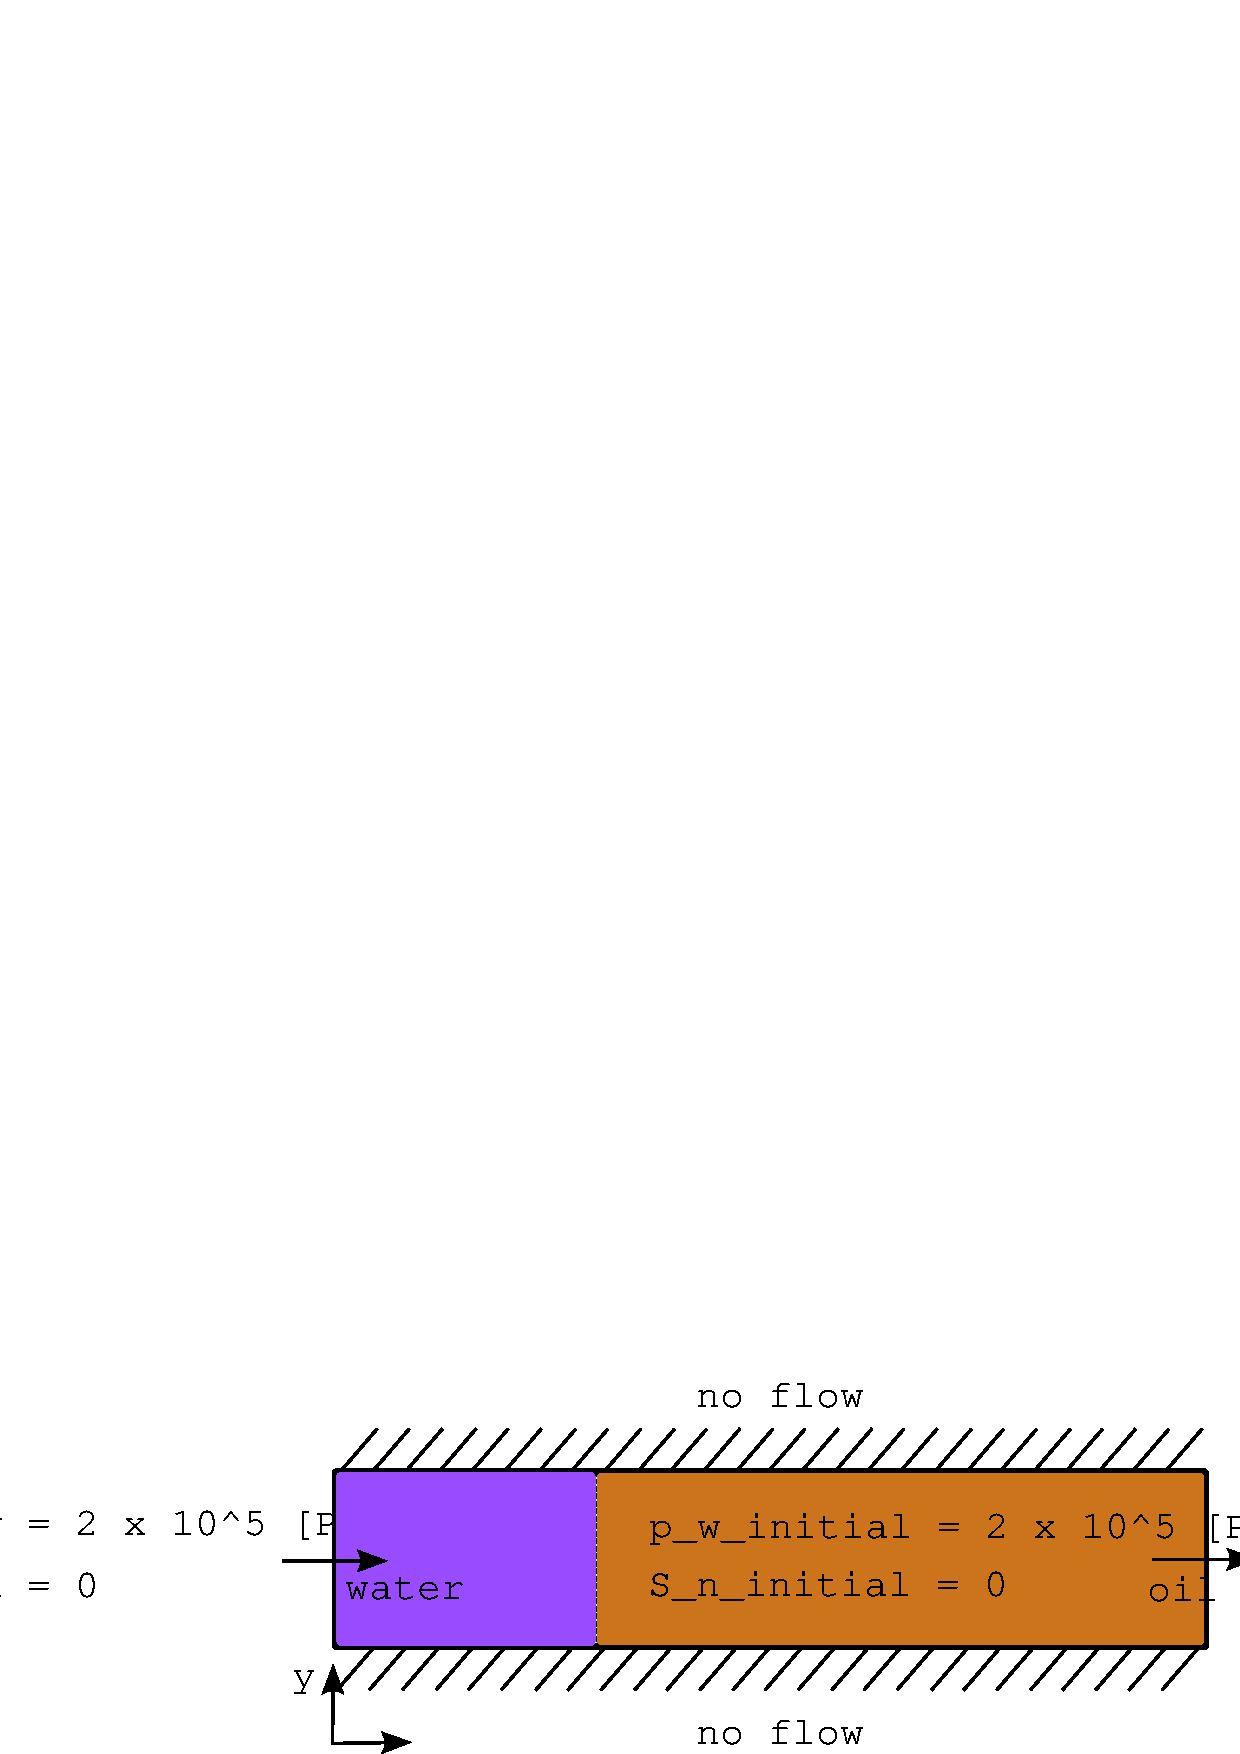
\includegraphics[width=0.9\linewidth,keepaspectratio]{EPS/tutorial-problemconfiguration}
\caption{Geometry of the tutorial problem with initial and boundary conditions.}\label{tutorial-coupled:problemfigure}
\end{figure}

The solved equations are the mass balances of water and oil:
\begin{align}
  \label{massbalancewater}
  \frac {\partial (\phi \, S_{w}\, \varrho_{w})}{\partial t}
  -
  \nabla \cdot \left( \varrho_{w} \, \frac{k_{rw}}{\mu_{w}} \, \mathbf{K}\;\nabla p_w \right)
  -
  q_w
  & =
  0 \\
  \label{massbalanceoil}
  \frac {\partial (\phi \, S_{o}\, \varrho_{o})}{\partial t}
  -
  \nabla \cdot \left( \varrho_{o} \, \frac{k_{ro}}{\mu_{o}} \, \mathbf{K}\;\nabla p_o \right)
  -
  q_o 
  & =
  0
\end{align}

\subsection{The Main File}

Listing \ref{tutorial-coupled:mainfile} shows the main application file
\texttt{tutorial/tutorial\_coupled.cc} for the coupled two-phase
model. This file has to be compiled and executed in order to solve the problem described
above.

\begin{lst}[File tutorial/tutorial\_coupled.cc]\label{tutorial-coupled:mainfile} \mbox{}
  \lstinputlisting[basicstyle=\ttfamily\scriptsize,numbers=left,
  numberstyle=\tiny, numbersep=5pt, firstline=29]{../../tutorial/tutorial_coupled.cc}
\end{lst}

From line \ref{tutorial-coupled:include-begin} to line
\ref{tutorial-coupled:include-end} the headers required are included.

At line \ref{tutorial-coupled:set-type-tag} the type tag of the
problem, which is going to be simulated, is specified. All other data
types can be retrieved via the \Dumux property system and only depend
on this single type tag. For a more thourough introduction to the
\Dumux property system, see chapter~\ref{sec:propertysystem}.

After this \Dumux' default startup routine is called on line
\ref{tutorial-coupled:call-start}. To provide an error message, the
usage message which is displayed to the user if the simulation is
called incorrectly, is printed via the custom function which is defined
on line~\ref{tutorial-coupled:usage-function}. 

In this function the usage message is customized to the problem at hand. This means that at least the necessary parameters are listed here.  For more information about the input file please refer to section \ref{sec:inputFiles}.

\subsection{The Problem Class}

When solving a problem using \Dumux, the most important file is the
so-called \textit{problem file} as shown in
listing~\ref{tutorial-coupled:problemfile}.

\begin{lst}[File tutorial/tutorialproblem\_coupled.hh]\label{tutorial-coupled:problemfile} \mbox{}
\lstinputlisting[basicstyle=\ttfamily\scriptsize,numbers=left,
numberstyle=\tiny, numbersep=5pt, firstline=28]{../../tutorial/tutorialproblem_coupled.hh}
\end{lst}

First, a new type tag is created for the problem in line
\ref{tutorial-coupled:create-type-tag}.  In this case, the new type
tag inherits all properties from the \texttt{BoxTwoP} type tag, which
means that for this problem the two-phase box model is chosen as
discretization scheme. Further, it inherits from the spatial
parameters type tag, which is defined in the problem-dependent spatial
parameters file (line
\ref{tutorial-coupled:define-spatialparameters-typetag}).  On line
\ref{tutorial-coupled:set-problem}, a problem class is attached to the
new type tag, while the grid which is going to be used is defined in
line \ref{tutorial-coupled:set-grid} -- in this case that is
\texttt{Dune::YaspGrid}.  Since there's no uniform mechanism to
allocate grids in \Dune, \Dumux features the concept of grid creators.
In this case the generic \texttt{CubeGridCreator} which creates a
structured hexahedron grid of a specified size and resolution. For
this grid creator the  physical domain of the grid is specified via the
run-time parameters \texttt{Grid.upperRightX},
\texttt{Grid.upperRightY}, \texttt{Grid.numberOfCellsX} and
\texttt{Grid.numberOfCellsY}. These parameters can be specified via
the command-line or in a parameter file,
see~\ref{tutorial-coupled:runtime-parameters}.

Next, the appropriate fluid system, which specifies the thermodynamic
relations of the fluid phases, has to be chosen. By default, the
two-phase model uses the \texttt{TwoPImmiscibleFluidSystem}, which
assumes immiscibility of the phases, but requires that the components
used for the wetting and non-wetting phases to be explicitly set. In
this case, liquid water which uses the relations from
IAPWS'97~\cite{IAPWS1997} is chosen as the wetting phase on line
\ref{tutorial-coupled:wettingPhase} and liquid oil is chosen as the
non-wetting phase on line \ref{tutorial-coupled:nonwettingPhase}. The
last property, which is set in line \ref{tutorial-coupled:gravity},
tells the model not to use gravity.

Parameters which are specific to a physical set-up to be simulated,
such as boundary and initial conditions, source terms or temperature
within the domain, and which are required to solve the differential
equations of the models are specified via a \textit{problem} class. If
the two-phase box model is used, this class should be derived from
\texttt{TwoPBoxProblem} as done in line
\ref{tutorial-coupled:def-problem}.

The problem class always has at least five methods:
\begin{itemize}
\item A method \texttt{boundaryTypes()} specifying the type of
  boundary conditions at each vertex.
\item A method \texttt{dirichlet()} specifying the actual values for
  the \textsc{Dirichlet} conditions at each \textsc{Dirichlet} vertex.
\item A method \texttt{neumann()} specifying the actual values for
  the \textsc{Neumann} conditions, which are usually evaluated at the 
  integration points of the \textsc{Neumann} boundary faces.
\item A method for source or sink terms called \texttt{source()}, usually evaluated at
  the center of a control volume.
\item A method called \texttt{initial()} for specifying the initial
  conditions at each vertex.
\end{itemize}

For the definition of the the boundary condition types and of the
values of the \textsc{Dirichlet} boundaries, two parameters are
available:
\begin{description}
 \item [values:]  A vector which stores the result of the method. What
  the values in this vector mean is dependent on the method: For
  \texttt{dirichlet()} it contains the actual values of the primary
  variables, for \texttt{boundaryTypes()} it contains the boundary 
  condition types. It has as many entries as the model has primary variables / equations.
  For the typical case, in which all equations have the same boundary
  condition type at a certain position, there are two methods that set the appropriate conditions
  for all primary variables / equations: \texttt{setAllDirichlet()} and \texttt{setAllNeumann()}.
\item [vertex:] The boundary condition and the Dirichlet values are
  specified for a vertex, which represents a control volume in the box
  discretization. This avoids the specification of two different
  boundary condition types for one equation at different control
  volume.  Be aware that the second parameter is a Dune grid entity
  with the codimension \texttt{dim}.
\end{description}

To ensure that no boundaries are undefined, a small safeguard value
\texttt{eps\_} is usually added when comparing spatial
coordinates. The left boundary is hence detected by comparing the
first coordinate is equal with zero, but by testing whether it is
smaller than a very small value \texttt{eps\_}.

Methods which make statements about boundary segments of the grid
(i.e.  \texttt{neumann()}) get called with six arguments:
\begin{description}
\item[values:] A vector \texttt{neumann()}, in which the mass fluxes per area unit
  over the boundary segment are specified.
\item[element:] The element of the grid where the boundary segment
  is located.
\item[fvElemGeometry:] The finite-volume geometry induced on the
  finite element by the box scheme.
\item[isIt:] The \texttt{Intersection} of the boundary segment as given by the grid.
\item[scvIdx:] The index of the sub-control volume in
  \texttt{fvElementGeometry} adjacent to the boundary segment.
\item[boundaryFaceIdx:] The index of the boundary face in
  \texttt{fvElementGeometry} which represents the boundary segment.  
\end{description}

Similarly, the \texttt{initial()} and \texttt{source()} methods
specify properties of control volumes and thus only get
\texttt{values}, \texttt{element}, \texttt{fvElemGeom} and
\texttt{scvIdx} as arguments.

In addition to these five methods, there might be some model-specific
methods. If the isothermal two-phase model is used, this includes for
example a \texttt{temperature()} method which returns the temperature
in \textsc{Kelvin} of the fluids and the rock matrix in the
domain. This temperature is then used by the model to calculate fluid
properties which possibly depend on it, e.g. density. The
\texttt{bboxMax()} (``\textbf{max}imum coordinated of the grid's
\textbf{b}ounding \textbf{b}ox'') method that is used here to
determine the extend of the phsical domain, returns a vector with the
maximum values of each coordinate of the grid's physical. This method
and the analogous \texttt{bboxMin()} method are provided by the base
class \texttt{Dumux::BoxProblem<TypeTag>}.

\subsection{Defining Fluid Properties}\label{tutorial-coupled:description-fluid-class}

The \Dumux distribution includes some common substances which can be
used out of the box. The properties of the pure substances (such as
the components nitrogen, water, or the pseudo-component air) are
provided by header files located in the folder
\verb+dumux/material/components+.

Most often, when two or more components are considered, fluid
interactions such as solubility effects come into play and properties
of mixtures such as density or enthalpy are of interest. These
interactions are defined by {\em fluid systems}, which are located in
\verb+dumux/material/fluidsystems+. A more thorough overview of the
\Dumux fluid framework can be found in chapter~\ref{sec:fluidframework}.

% In this example, a class for the definition of a two-phase system is used. This allows for the choice 
% of the two components oil and water and for access of the parameters that are relevant for the two-phase model.

\subsection{Definiting Spatially Dependent Parameters}\label{tutorial-coupled:description-spatialParameters}

In \Dumux, many properties of the porous medium can depend on the
spatial location. Such properties are the \textit{intrinsic
  permeability}, the parameters of the \textit{capillary pressure} and
the \textit{relative permeability}, the \textit{porosity}, the
\textit{heat capacity} as well as the \textit{heat conductivity}. Such
parameters are define using a so-called \textit{spatial parameters}
class.

The the box discretization is to be used, the spatial paramters class
should be derived from the base class
\texttt{Dumux::BoxSpatialParameters<TypeTag>}. Listing
\ref{tutorial-coupled:spatialparametersfile} shows the file
\verb+tutorialspatialparameters_coupled.hh+:

\begin{lst}[File tutorial/tutorialspatialparameters\_coupled.hh]\label{tutorial-coupled:spatialparametersfile} \mbox{}
\lstinputlisting[basicstyle=\ttfamily\scriptsize,numbers=left,
numberstyle=\tiny, numbersep=5pt, firstline=28]{../../tutorial/tutorialspatialparameters_coupled.hh}
\end{lst}

First, the spatial parameters type tag is created on line
\ref{tutorial-coupled:define-spatialparameters-typetag}. The type tag
for the problem then derives from it. The \Dumux properties defined on
the type tag for the spatial parameters are for example, the spatial
parameters class itself (line
\ref{tutorial-coupled:set-spatialparameters}) or the capillary
pressure/relative permability relations\footnote{Taken together, the
  capillary pressure and the relative permeability relations are
  called \textit{material law}.} which ought to be used by the
simulation (line
\ref{tutorial-coupled:rawlaw} \label{tutorial-coupled:materialLaw}).
\Dumux provides several material laws in the folder
\verb+dumux/material/fluidmatrixinteractions+.  The selected one --
here it is a relation according to a regularized version of
\textsc{Brooks} \& \textsc{Corey} -- is included in line
\ref{tutorial-coupled:rawLawInclude}. After the selection, an adapter
class is specified ob line \ref{tutorial-coupled:eff2abs} to
translates between effective and absolute saturations. This way,
residual saturations can be specified in a generic way.  As only used
material law knows which the names of the parameters which it
requires, it provides a parameter class
\texttt{RegularizedBrooksCoreyParams} which is exported by the type
\texttt{Params} and defined in line
\ref{tutorial-coupled:matLawObjectType}. In this case, the spatial
parameters only require a single set of parameters which means that it
only requires a single material parameter object as can be seen on
line~\ref{tutorial-coupled:matParamsObject}.

In line \ref{tutorial-coupled:permeability}, a method returning the
intrinsic permeability is specified. As can be seen, the method has
to be called with three arguments:
\begin{description}
\item[\texttt{element}:] Just like for the problem itself, this
  parameter describes the considered element by means of a \Dune
  entity. Elements provide information about its geometry and
  position and can be mapped to a global index.
\item[\texttt{fvElemGeom}:] Holds information about the finite-volume
  geometry induced by the box-method on the element.
\item[\texttt{scvIdx}:] Is the index of the sub-control volume of the
  element which is considered. This is equivalent to the local index
  of the vertex which corrosponts to the considered control volume in
  the element.
\end{description}

The intrinsic permeability is a tensor and is thus the method returnes
a $\texttt{dim} \times \texttt{dim}$-matrix where \texttt{dim} is the
dimension of the grid.

The method \texttt{porosity()} defined in line
\ref{tutorial-coupled:porosity} is called with the same arguments as
\texttt{intrinsicPermeability()} and returns a scalar value for
porosity dependent on the position in the domain.

Next, the method \texttt{materialLawParams()}, defined on line
\ref{tutorial-coupled:matLawParams}, specifies
\verb+materialLawParams+ object applies at the specified
position. Although in this case only one object is returned, in
general, the problem may be heterogeneous, which necessitates
returning different objects at different positions in space.  While
the selection of the type of this object was already explained (line
\ref{tutorial-coupled:rawLawInclude}), some specific parameter values
of the used material law, such as the \textsc{Brooks} \&
\textsc{Corey} parameters, are still needed. This is done in the
constructor at line \ref{tutorial-coupled:setLawParams}.  Depending on
the type of the \texttt{materialLaw} object, the \texttt{set}-methods
might be different than those given in this example. The name of the
access / set functions as well as the rest of the implementation of
the material description can be found in
\verb+dumux/material/fluidmatrixinteractions/2p+.

\subsection{Definition of Run-Time Parameters}\label{tutorial-coupled:runtime-parameters}

Some parameters need to be specified at runtime. These can either be
specified directly via command line optioms or they can be collected in
a parameter file. The parameter file which \Dumux uses by default has
the name of the program with ``.input'' appended. The parameter file
for the coupled tutorial is thus named \verb+tutorial_coupled.input+
and has the content shown in listing~\ref{tutorial-coupled:parameter-file}.

\begin{lst}[File tutorial/tutorial\_coupled.input]\label{tutorial-coupled:parameter-file} \mbox{}
\lstinputlisting[basicstyle=\ttfamily\scriptsize,numbers=left,numberstyle=\tiny]{../../tutorial/tutorial_coupled.input}
\end{lst}

\subsection{Exercises}
\label{tutorial-coupled:exercises}
The following exercises will give you the opportunity to learn how you
can change soil parameters, boundary conditions, run-time parameters
and fluid properties in \Dumux.

\subsubsection{Exercise 1}
\renewcommand{\labelenumi}{\alph{enumi})} For Exercise 1 you have
to make only some small changes in the tutorial files.  

\begin{enumerate}

\item \textbf{Running the Program} \\
  To get an impression what the results should look like you can first run the original version of the coupled tutorial model by typing  \texttt{./tutorial\_coupled}. Note, that the time-step size is automatically adapted during the simulation. For the visualization of the results using paraview please refer to section \ref{quick-start-guide}.\\

\item \textbf{Changing the Model Domain and the Boundary Conditions} \\
  Change the size of the model domain so that you get a rectangle with
  edge lengths of $\text{x} = 400 m$ and $\text{y} = 500 m$ and with
  discretization lengths of $\Delta \text{x} = 20$ m and $\Delta
  \text{y} = 20$ m.
  
  Change the boundary conditions in the file
  \texttt{tutorialproblem\_coupled.hh} so that water enters from the
  bottom and oil is extracted from the top boundary. The right and the
  left boundary should be closed for water and oil fluxes. 

  Compile the main file by typing \texttt{make tutorial\_coupled} and
  run the model as explained above.

\item \textbf{Changing Fluids} \\
Now you can change the fluids. Use DNAPL instead of Oil and Brine instead of Water. To do that, you have to select different components via the property system in the problem file:
\begin{enumerate}
 \item Brine: Brine is thermodynamically very similar to pure water but also considers a fixed amount of salt in the liquid phase. Hence, the class \texttt{Dumux::Brine} uses a pure water class, such as \texttt{Dumux::H2O}, as a second template argument after the data type \texttt{<Scalar>} as a template argument.
 \item DNAPL: A standard set of chemical substances, such as Oil and Brine, is already included in the problem (via a list of \texttt{\#include ..} statements) and hence easily accessible by default. However, this is not the case for the class \texttt{Dumux::SimpleDNAPL}, which describes a simple \textbf{d}ense \textbf{n}on-\textbf{a}queous \textbf{p}hase \textbf{l}iquid and is located in the folder \texttt{dumux/material/components/}. Try to include the file and select the component as the non-wetting phase via the property system.
\end{enumerate}
If you want to take a closer look on how the fluid classes are defined and which substances are already available please browse through the files in the directory
\texttt{/dumux/material/components} and read chapter~\ref{sec:fluidframework}.

\item \textbf{Use a Full-Fledged Fluid System} \\
\Dumux usually describes fluid mixtures via \textit{fluid systems}, see also chapter \ref{sec:fluidframework}. In order to include a fluid system, you first have to comment out lines \ref{tutorial-coupled:2p-system-start} to \ref{tutorial-coupled:2p-system-end} in the problem file. If you use eclipse, this can easily be done by pressing \textit{Ctrl + Shift + 7} -- the same as to cancel the comment later on.\\
Now include the file \texttt{fluidsystems/h2oairsystem.hh} in the material folder, and set a property \texttt{FluidSystem} with the appropriate type, i.e. \texttt{Dumux::H2OAirFluidSystem<TypeTag>}. However, this is a rather complicated fluid system considers mixtures of components and also uses tabulated components that need to be initialized -- i.e. the tables need to be filled with values. Initializating the fluid system is normally done in the constructor of the problem by calling \texttt{GET\_PROP\_TYPE(TypeTag, FluidSystem)::init();}. As water flow replacing a gas is much faster, test your simulation only until $2000$ seconds and start with a time step of $1$ second.\\
Please reverse the changes made in this part of the exercise, as we will continue to use immiscible phases from here on and hence do not need a complex fluid system.

\item \textbf{Changing Constitutive Relations} \\
  Use an unregularized linear law with an entry pressure of $p_e = 0.0\;\text{Pa}$ and maximal capillary pressure of e.g. $p_{c_{max}} = 2000.0\;\text{Pa}$ instead of using a
 regularized Brooks-Corey law for the
  relative permeability and for the capillary pressure saturation relationship. To do that you have
  to change the file \texttt{tutorialspatialparameters\_coupled.hh}. 
 You can find the material laws in the folder 
  \verb+dumux/material/fluidmatrixinteractions+. The necessary parameters
of the linear law and the respective \texttt{set}-functions can be found
 in the file \\
 \verb+dumux/material/fluidmatrixinteractions/2p/linearmaterialparams.hh+.
 
\item \textbf{Heterogeneities}  \\
  Set up a model domain with the soil properties given in Figure
  \ref{tutorial-coupled:exercise1_d}. Adjust the boundary conditions
  so that water is again flowing from the left to the right of the
\begin{figure}[ht]
\psfrag{K1 =}{$\mathbf{K} = 10^{-8}\;\text{m}^2$}
\psfrag{phi1 =}{$\phi = 0.15$}
\psfrag{K2 =}{\textcolor{white}{$\mathbf{K} = 10^{-9}\;\text{m}^2$}}
\psfrag{phi2 =}{\textcolor{white}{$\phi = 0.3$}}
\psfrag{600 m}{$600 \;\text{m}$}
\psfrag{300 m}{$300 \;\text{m}$}
\centering
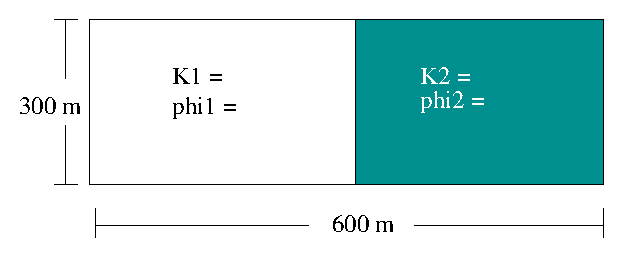
\includegraphics[width=0.5\linewidth,keepaspectratio]{EPS/exercise1_c.eps}
\caption{Exercise 1f: Set-up of a model domain with a heterogeneity. $\Delta x = 20 \;\text{m}$ $\Delta y = 20\;\text{m}$.}\label{tutorial-coupled:exercise1_d}
\end{figure}
domain. You can use the fluids of exercise 1c).\\
\textbf{Hint:} The current position of the control volume can be obtained using \texttt{element\allowbreak.geometry()\allowbreak.corner(scvIdx)}.\\
When does the front cross the material border? In paraview, the
animation view (\textit{View} $\rightarrow$ \textit{Animation
  View}) is a convenient way to get a rough feeling of the time-step
sizes.
\end{enumerate}

\subsubsection{Exercise 2}
For this exercise you should create a new problem file analogous to
the file \texttt{tutorialproblem\_coupled.hh} (e.g. with the name
\texttt{ex2\_tutorialproblem\_coupled.hh} and new spatial parameters
just like \texttt{tutorialspatialparameters\_coupled.hh}. The new
problem file needs to
be included in the file \texttt{tutorial\_coupled.cc}.\\
The new files should contain the definition of new classes with names
that relate to the file name, such as
\texttt{Ex2TutorialProblemCoupled}. Make sure that you also adjust the
guardian macros in lines \ref{tutorial-coupled:guardian1} and
\ref{tutorial-coupled:guardian1}
in the header files (e.g. change \\
\texttt{DUMUX\_TUTORIALPROBLEM\_COUPLED\_HH} to
\texttt{DUMUX\_EX2\_TUTORIALPROBLEM\_COUPLED\_HH}). Besides also
adjusting the guardian macros, the new problem file should define and
use a new type tag for the problem as well as a new problem class
e.g. \texttt{Ex2TutorialProblemCoupled}. Make sure to assign your
newly defined spatial parameter class to the
\texttt{SpatialParameters} property for the new
type tag. \\
After this, change the run-time parameters so that they match the
domain described by figure \ref{tutorial-coupled:ex2_Domain}. Adapt
the problem class so that the boundary conditions are consistent with
figure \ref{tutorial-coupled:ex2_BC}. Initially, the domain is fully
saturated with water and the pressure is $p_w = 5 \times
10^5\;\text{Pa}$.  Oil infiltrates from the left side. Create a grid
with $20$ cells in $x$-direction and $10$ cells in $y$-direction. The
simulation time should be set to $10^6\;\text{s}$ with an
initial time step size of $100\;\text{s}$.

Now include your new problem file in the main file and replace the
\texttt{TutorialProblemCoupled} type tag by the one you've created and
compile the program.


\begin{figure}[ht]
\psfrag{K1}{K $= 10^{-7}\;\text{m}^2$}
\psfrag{phi1}{$\phi = 0.2$}
\psfrag{Lin}{Brooks-Corey Law}
\psfrag{Lin2}{$\lambda = 1.8$, $p_e = 1000\;\text{Pa}$}
\psfrag{K2}{K $= 10^{-9}\;\text{m}^2$}
\psfrag{phi2}{$\phi = 0.15$}
\psfrag{BC1}{\textsc{Brooks}-\textsc{Corey} Law} 
\psfrag{BC2}{$\lambda = 2$, $p_e = 1500\;\text{Pa}$}
\psfrag{H1y}{$50\;\text{m}$}
\psfrag{H2y}{$15\;\text{m}$}
\psfrag{H3y}{$20\;\text{m}$}
\psfrag{L1x}{$100\;\text{m}$}
\psfrag{L2x}{$50\;\text{m}$}
\psfrag{L3x}{$25\;\text{m}$}
\centering
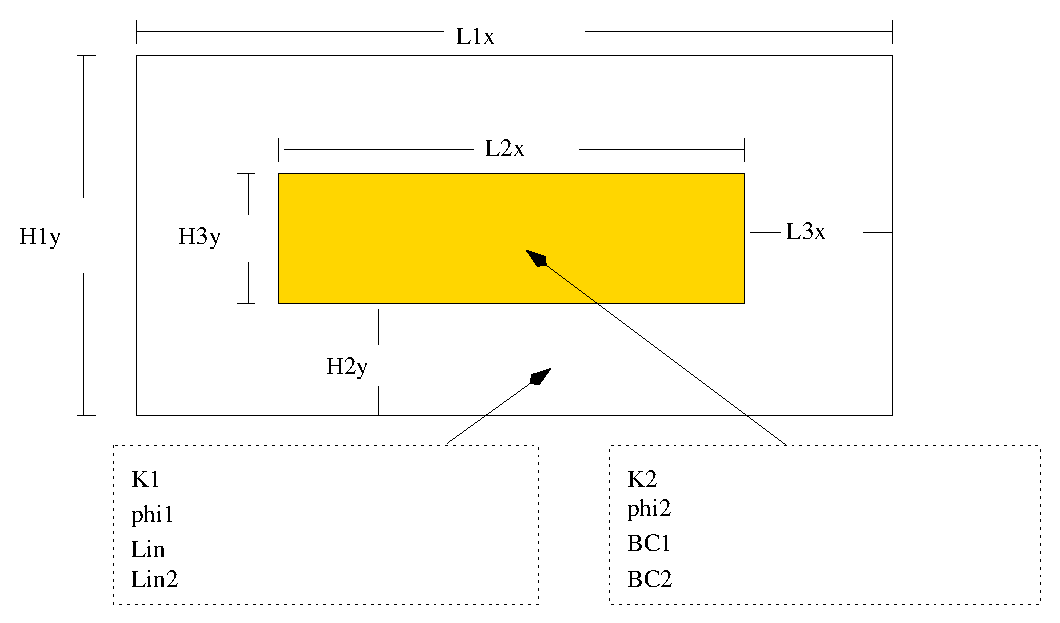
\includegraphics[width=0.8\linewidth,keepaspectratio]{EPS/Ex2_Domain.eps}
\caption{Set-up of the model domain and the soil parameters}\label{tutorial-coupled:ex2_Domain}
\end{figure}

\begin{figure}[ht]
\psfrag{pw}{$p_w = 5 \times 10^5\;\text{Pa}$}
\psfrag{S}{$S_n = 1.0$}
\psfrag{qw}{$q_w = 2 \times 10^{-4} \;\text{kg}/\text{m}^2\text{s}$}
\psfrag{qo}{$q_n = 0.0 \;\text{kg}/\text{m}^2\text{s}$}
\psfrag{no flow}{no flow}
\centering
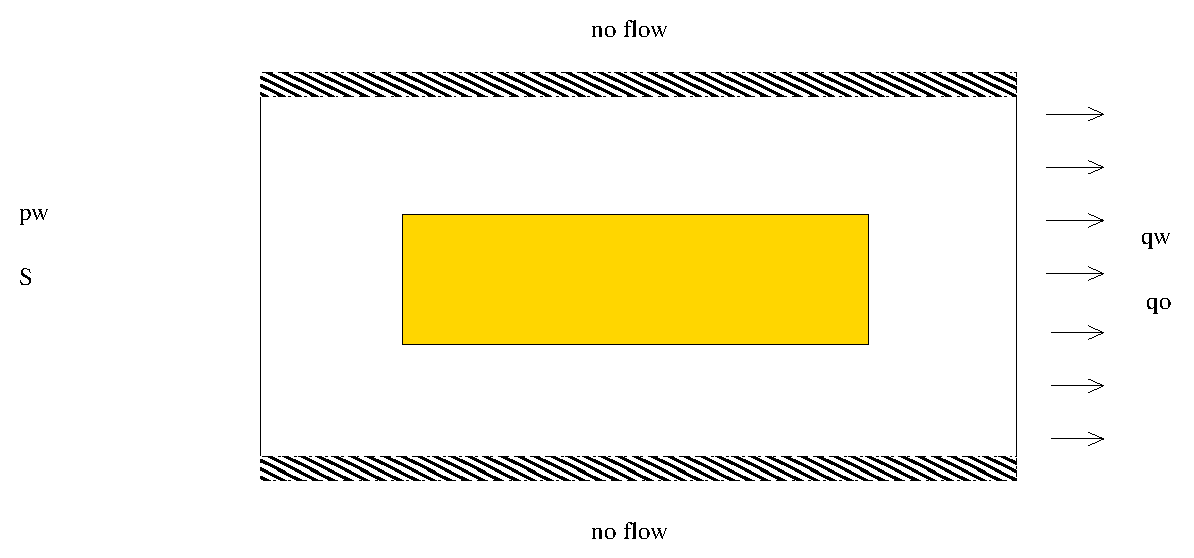
\includegraphics[width=0.8\linewidth,keepaspectratio]{EPS/Ex2_Boundary.eps}
\caption{Boundary Conditions}\label{tutorial-coupled:ex2_BC}
\end{figure}

\begin{itemize}
 \item Increase the simulation time to e.g. $4\times 10^7 \;\text{s}$. Investigate the saturation: Is the value range reasonable?
 \item What happens if you increase the resolution of the grid?
\end{itemize}

\subsubsection{Exercise 3: Parameter File Input}

As you have experienced, compilation takes quite some time. Therefore,
\Dumux provides a simple method to read in parameters at run-time
via \textit{paramter input files}.\\

In the code, parameters can be read via the macro
\texttt{GET\_RUNTIME\_PARAM(TypeTag, Scalar,
  MyWonderfulGroup.MyWonderfulParameter);}. At the end of the
simulation a list of parameters is printed if the command line option
\texttt{-printParams 1} is passed to the simulation. Add some (for
example \texttt{Newton.MaxSteps} and \texttt{EnableGravity}) to the
parameter file \texttt{tutorial\_coupled.input} and observe what
happens if they are modified. For more information about the input file please refer to section \ref{sec:inputFiles}.

\subsubsection{Exercise 4: Create a New Component}

Create a new file for the benzene component called \texttt{benzene.hh}
and implement a new component. (You may get a hint by looking at
existing fluid systems in the directory \verb+/dumux/material/components+). \\
Use benzene as a new fluid and run the model of Exercise 2 with water
and benzene. Benzene has a density of $889.51 \, \text{kg} /
\text{m}^3$ and a viscosity of $0.00112 \, \text{Pa} \; \text{s}$.

\clearpage \newpage
%%% Local Variables: 
%%% mode: latex
%%% TeX-master: "dumux-handbook"
%%% End: 
